\documentclass[9pt,twocolumn,twoside]{pnas-new}\usepackage[]{graphicx}\usepackage[]{color}
%% maxwidth is the original width if it is less than linewidth
%% otherwise use linewidth (to make sure the graphics do not exceed the margin)
\makeatletter
\def\maxwidth{ %
  \ifdim\Gin@nat@width>\linewidth
    \linewidth
  \else
    \Gin@nat@width
  \fi
}
\makeatother

\definecolor{fgcolor}{rgb}{0.345, 0.345, 0.345}
\newcommand{\hlnum}[1]{\textcolor[rgb]{0.686,0.059,0.569}{#1}}%
\newcommand{\hlstr}[1]{\textcolor[rgb]{0.192,0.494,0.8}{#1}}%
\newcommand{\hlcom}[1]{\textcolor[rgb]{0.678,0.584,0.686}{\textit{#1}}}%
\newcommand{\hlopt}[1]{\textcolor[rgb]{0,0,0}{#1}}%
\newcommand{\hlstd}[1]{\textcolor[rgb]{0.345,0.345,0.345}{#1}}%
\newcommand{\hlkwa}[1]{\textcolor[rgb]{0.161,0.373,0.58}{\textbf{#1}}}%
\newcommand{\hlkwb}[1]{\textcolor[rgb]{0.69,0.353,0.396}{#1}}%
\newcommand{\hlkwc}[1]{\textcolor[rgb]{0.333,0.667,0.333}{#1}}%
\newcommand{\hlkwd}[1]{\textcolor[rgb]{0.737,0.353,0.396}{\textbf{#1}}}%
\let\hlipl\hlkwb

\usepackage{framed}
\makeatletter
\newenvironment{kframe}{%
 \def\at@end@of@kframe{}%
 \ifinner\ifhmode%
  \def\at@end@of@kframe{\end{minipage}}%
  \begin{minipage}{\columnwidth}%
 \fi\fi%
 \def\FrameCommand##1{\hskip\@totalleftmargin \hskip-\fboxsep
 \colorbox{shadecolor}{##1}\hskip-\fboxsep
     % There is no \\@totalrightmargin, so:
     \hskip-\linewidth \hskip-\@totalleftmargin \hskip\columnwidth}%
 \MakeFramed {\advance\hsize-\width
   \@totalleftmargin\z@ \linewidth\hsize
   \@setminipage}}%
 {\par\unskip\endMakeFramed%
 \at@end@of@kframe}
\makeatother

\definecolor{shadecolor}{rgb}{.97, .97, .97}
\definecolor{messagecolor}{rgb}{0, 0, 0}
\definecolor{warningcolor}{rgb}{1, 0, 1}
\definecolor{errorcolor}{rgb}{1, 0, 0}
\newenvironment{knitrout}{}{} % an empty environment to be redefined in TeX

\usepackage{alltt}
% Use the lineno option to display guide line numbers if required.

\templatetype{pnasresearcharticle} % Choose template 

\title{Forecasting seasonal influenza in the U.S.: A collaborative multi-year, multi-model assessment of forecast performance}

\author[a]{Nicholas G Reich}
\author[b]{Logan Brooks}
\author[c]{Spencer Fox}
\author[d]{Sasikiran Kandula}
\author[e]{Craig McGowan}
\author[a]{Evan Moore}
\author[f]{Dave Osthus}
\author[g]{Evan L Ray}
\author[a]{Abhinav Tushar}
\author[d]{Teresa Yamana}
\author[e]{Matthew Biggerstaff}
\author[h]{Michael A Johansson}
\author[i]{Roni Rosenfeld}
\author[d]{Jeffrey Shaman}

\affil[a]{Department of Biostatistics and Epidemiology, University of Massachusetts-Amherst, Amherst, 01003, USA}
\affil[b]{Department of Computer Science, Carnegie Mellon University, Pittsburgh,  USA}
\affil[c]{University of Texas at Austin, Austin, USA}
\affil[d]{Columbia University, New York, USA}
\affil[e]{Influenza Division, Centers for Disease Control and Prevention, Atlanta, USA}
\affil[f]{Los Alamos National Laboratory, Los Alamos, USA}
\affil[g]{Mount Holyoke College, South Hadley, USA}
\affil[h]{Division of Vector-Borne Diseases, Centers for Disease Control and Prevention, Atlanta, USA}
\affil[i]{Department of Machine Learning, Carnegie Mellon University, Pittsburgh,  USA}

\leadauthor{Reich} 

\significancestatement{Accurate prediction of the size and timing of infectious disease outbreaks could help public health officials in planning an appropriate response. This paper compares approaches developed by five different research groups to forecast seasonal influenza outbreaks in real-time in the US. Many of the models show more accurate forecasts than a historical baseline. A major impediment to predictive ability was the real-time accuracy of available data. The field of infectious disease forecasting is in its infancy and we expect that innovation will spur improvements in forecasting in the coming years.}

\authorcontributions{All authors designed the research; N.G.R., L.B., S.F., S.K., C.M., E.M., D.O., E.L.R., A.T., T.Y. performed research by implementing the models; N.G.R., C.M., E.M. analyzed data; N.G.R. wrote the paper; all authors provided editorial feedback on the paper.}
\authordeclaration{JS and Columbia University disclose partial ownership of SK Analytics.}
%\equalauthors{\textsuperscript{1}A.O.(Author One) and A.T. (Author Two) contributed equally to this work (remove if not applicable).}
\correspondingauthor{\textsuperscript{2}To whom correspondence should be addressed. E-mail: nick\@schoolph.umass.edu}

\keywords{} 

 

% Overall character count must not exceed 49,000 characters for a 6-page article and 82,000 for a 10-page article; this includes text, spaces, and the number of characters displaced by figures, tables, and equations.
% Text: When submitting tables, figures, and/or equations in addition to text, keep the text for your manuscript under 5 two-column, single-spaced pages, or under 39,000 characters for a 6-page article and 65,000 for a 10-page article (including spaces).
% Figures: Calculated at 180 characters per cm in height for one column and 360 characters per cm in height for two columns.
% Tables and equations: Calculated at 60 characters per line for one column and 120 characters per line for two columns.

\begin{abstract}

% 250 word limit
Influenza infects an estimated 9 to 35 million individuals each year in the United States and is a contributing cause for between 12,000 and 56,000 deaths annually.
Seasonal outbreaks of influenza are common in temperate regions of the world, with highest incidence typically occurring in colder and drier months of the year. 
Real-time forecasts of influenza transmission can inform public health response to outbreaks. 
We present the results of a multi-institution collaborative effort to standardize the collection and evaluation of forecasting models for influenza in the US for the 2010/2011 through 2016/2017 influenza seasons. 
For these seven seasons, we assembled weekly real-time forecasts of 7 targets of public health interest from 22 different models.
We compared forecast accuracy of each model relative to a historical baseline seasonal average.
Across all regions of the US, over half of the models showed consistently better performance than the historical baseline when forecasting incidence of influenza-like illness 1, 2 and 3 weeks ahead of available data and when forecasting the timing and magnitude of the seasonal peak.
In some regions, delays in data reporting were strongly and negatively associated with forecast accuracy.
More timely reporting and an improved overall accessibility to novel and traditional data sources are needed to improve forecasting accuracy and its integration with real-time public health decision-making.

\end{abstract}

\dates{This manuscript was compiled on \today}
\doi{\url{www.pnas.org/cgi/doi/10.1073/pnas.XXXXXXXXXX}}
\IfFileExists{upquote.sty}{\usepackage{upquote}}{}
\begin{document}

\maketitle
\thispagestyle{firststyle}
\ifthenelse{\boolean{shortarticle}}{\ifthenelse{\boolean{singlecolumn}}{\abscontentformatted}{\abscontent}}{}




%\tableofcontents









\dropcap{O}ver the past 15 years, the number of published research articles on forecasting infectious diseases has tripled (Web of Science). 
This increased interest has been fueled in part by the promise of `big data', that near real-time data streams of information ranging from large-scale population behavior \cite{Molodecky2017} to microscopic changes in a pathogen \cite{Du2017} could lead to measurable improvements in how disease transmission is measured, forecasted, and controlled \cite{Bansal2016}. 
With the spectre of a global pandemic looming, improving infectious disease forecasting continues to be a central priority of global health preparedness efforts.\cite{Myers2000,WorldHealthOrganization2016,Chretien2015}

Forecasts of infectious disease transmission can inform public health response to outbreaks. 
Accurate forecasts of the timing and spatial spread of infectious disease incidence can provide valuable information about where public health interventions can be targeted.\cite{Lipsitch2011}
Decisions about hospital staffing, resource allocation, the timing of public health communication campaigns, and the implementation of interventions designed to disrupt disease transmission, such as vector control measures, can be informed by forecasts.
In part due to the growing recognition of the importance of systematically integrating forecasting into public health outbreak response, large-scale collaborations have been used in forecasting applications to develop common data standards and facilitate comparisons across multiple models.\cite{Biggerstaff2016,Smith2017,Biggerstaff2018,Viboud2017}
%These studies serve as an important counterweight to many forecasting efforts remain one-off academic exercises focused on a single application or a single method.
By enabling a standardized comparison in a single application, these studies greatly improve our understanding of which models perform best in certain settings, of how results can best be disseminated and used by decision-makers, and of what the bottlenecks are in terms of improving forecasts.

While multi-model comparisons exist in the literature for single-outbreak performance \cite{Biggerstaff2016,Viboud2017,Biggerstaff2018}, here we compare a consistent set of models over seven influenza seasons. 
To our knowledge, this is the first documented comparison of multiple real-time forecasting models from different teams across multiple seasons for any infectious disease application.
Since each season has a unique dynamical structure, multi-season comparisons like this have great potential to improve our understanding of how models perform over the long term and which models may be reliable in the future.

Influenza is a respiratory viral infection that can cause mild or severe symptoms.
In the US each year, influenza viruses infect an estimated 9 to 35 million individuals and cause between 12,000 and 56,000 deaths.\cite{Rolfes2016}
Influenza incidence typically exhibits a strong annual periodicity in the US (and in other global regions with temperate climates), often circulating widely during colder months (i.e., November through April). 
The social, biological, environmental, and demographic features that contribute to higher-than-usual incidence in a particular season are not fully understood, although contributing factors may include severity of the dominant influenza subtype\cite{thompson2003}, pre-existing population immunity due to prior infections or vaccination\cite{Woolthuis2017,Zarnitsyna2018}, temperature and humidity\cite{lowen2007}, vaccine effectiveness\cite{Rolfes2016}, or timing of school vacations\cite{cauchemez2008}.

%This work relies on the forecasting structure developed by existing public forecasting challenges.
Starting in the 2013/2014 influenza season, the U.S. Centers for Disease Control and Prevention (CDC) has run the ``Forecast the Influenza Season Collaborative Challenge'' (a.k.a. FluSight) each influenza season, soliciting prospective, real-time weekly forecasts of regional-level weighted influenza-like illness (wILI) measures from teams across the world (Figure \ref{fig:intro-schematic}).\cite{Biggerstaff2016,Biggerstaff2018}
The FluSight challenge focuses on forecasts of the weighted percentage of doctor's office visits where the patient showed symptoms of an influenza-like illness in a particular region. Weighting is done by state population as the data are aggregated to the regional and national level.
This wILI metric is a standard measure of seasonal flu activity, for which public data are available for the US back to the 1997/1998 influenza season (Figure \ref{fig:intro-schematic}A). 
The FluSight challenge forecasts are displayed together on a website in real-time and are evaluated for accuracy at the end of the season.\cite{PhiResearchLab} 
This effort has galvanized a community of scientists interested in forecasting, creating a testbed for improving both the technical understanding of how different forecast models perform and the integration of these models into decision-making.

%We present a standardized comparison of a range of different forecasting models for influenza in the US, over multiple seasons.
Building on the structure of the FluSight challenges (and those of other collaborative forecasting efforts \cite{Smith2017,Viboud2017}), a subset of FluSight participants formed a consortium in early 2017 to facilitate direct comparison and fusion of modeling approaches. 
Our work brings together 22 models from five different institutions: Carnegie Mellon University, Columbia University, Los Alamos National Laboratory, University of Massachusetts-Amherst, and University of Texas-Austin (Table \ref{tab:model-list}).
% While most groups developed more than one model for consideration, the models developed within a single group through the use of common data sources and/or methodologies often bear similarities to each other.
% Having models from different teams enhances the diversity of the models presented.
In this paper, we provide a detailed analysis of the performance of these different models in forecasting the targets defined by the CDC FluSight challenge organizers (Figure \ref{fig:intro-schematic}B).
Drawing on the different expertise of the five teams allows us to make fine-grained and standardized comparisons of distinct approaches to disease incidence forecasting that use different data sources and modeling frameworks.

In addition to analyzing comparative model performance over multiple seasons, this work identifies key bottlenecks that limit the accuracy and generalizability of current forecasting efforts.
Specifically, we present quantitative analyses of the impact that incomplete or partial case reporting has on forecast accuracy.
Additionally, we assess whether purely statistical models show similar performance to models that consider explicit mechanistic models of disease transmission.
Overall, this work shows strong evidence that carefully crafted forecasting models for region-level influenza in the US consistently outperformed a historical baseline model for targets of particular public health interest. 
%This collaboration from a subset of the core community of influenza forecasters in the US, and other collaborations like it, will continue to advance infectious disease forecasting capabilities globally. 

\begin{figure}[htbp]
\centering
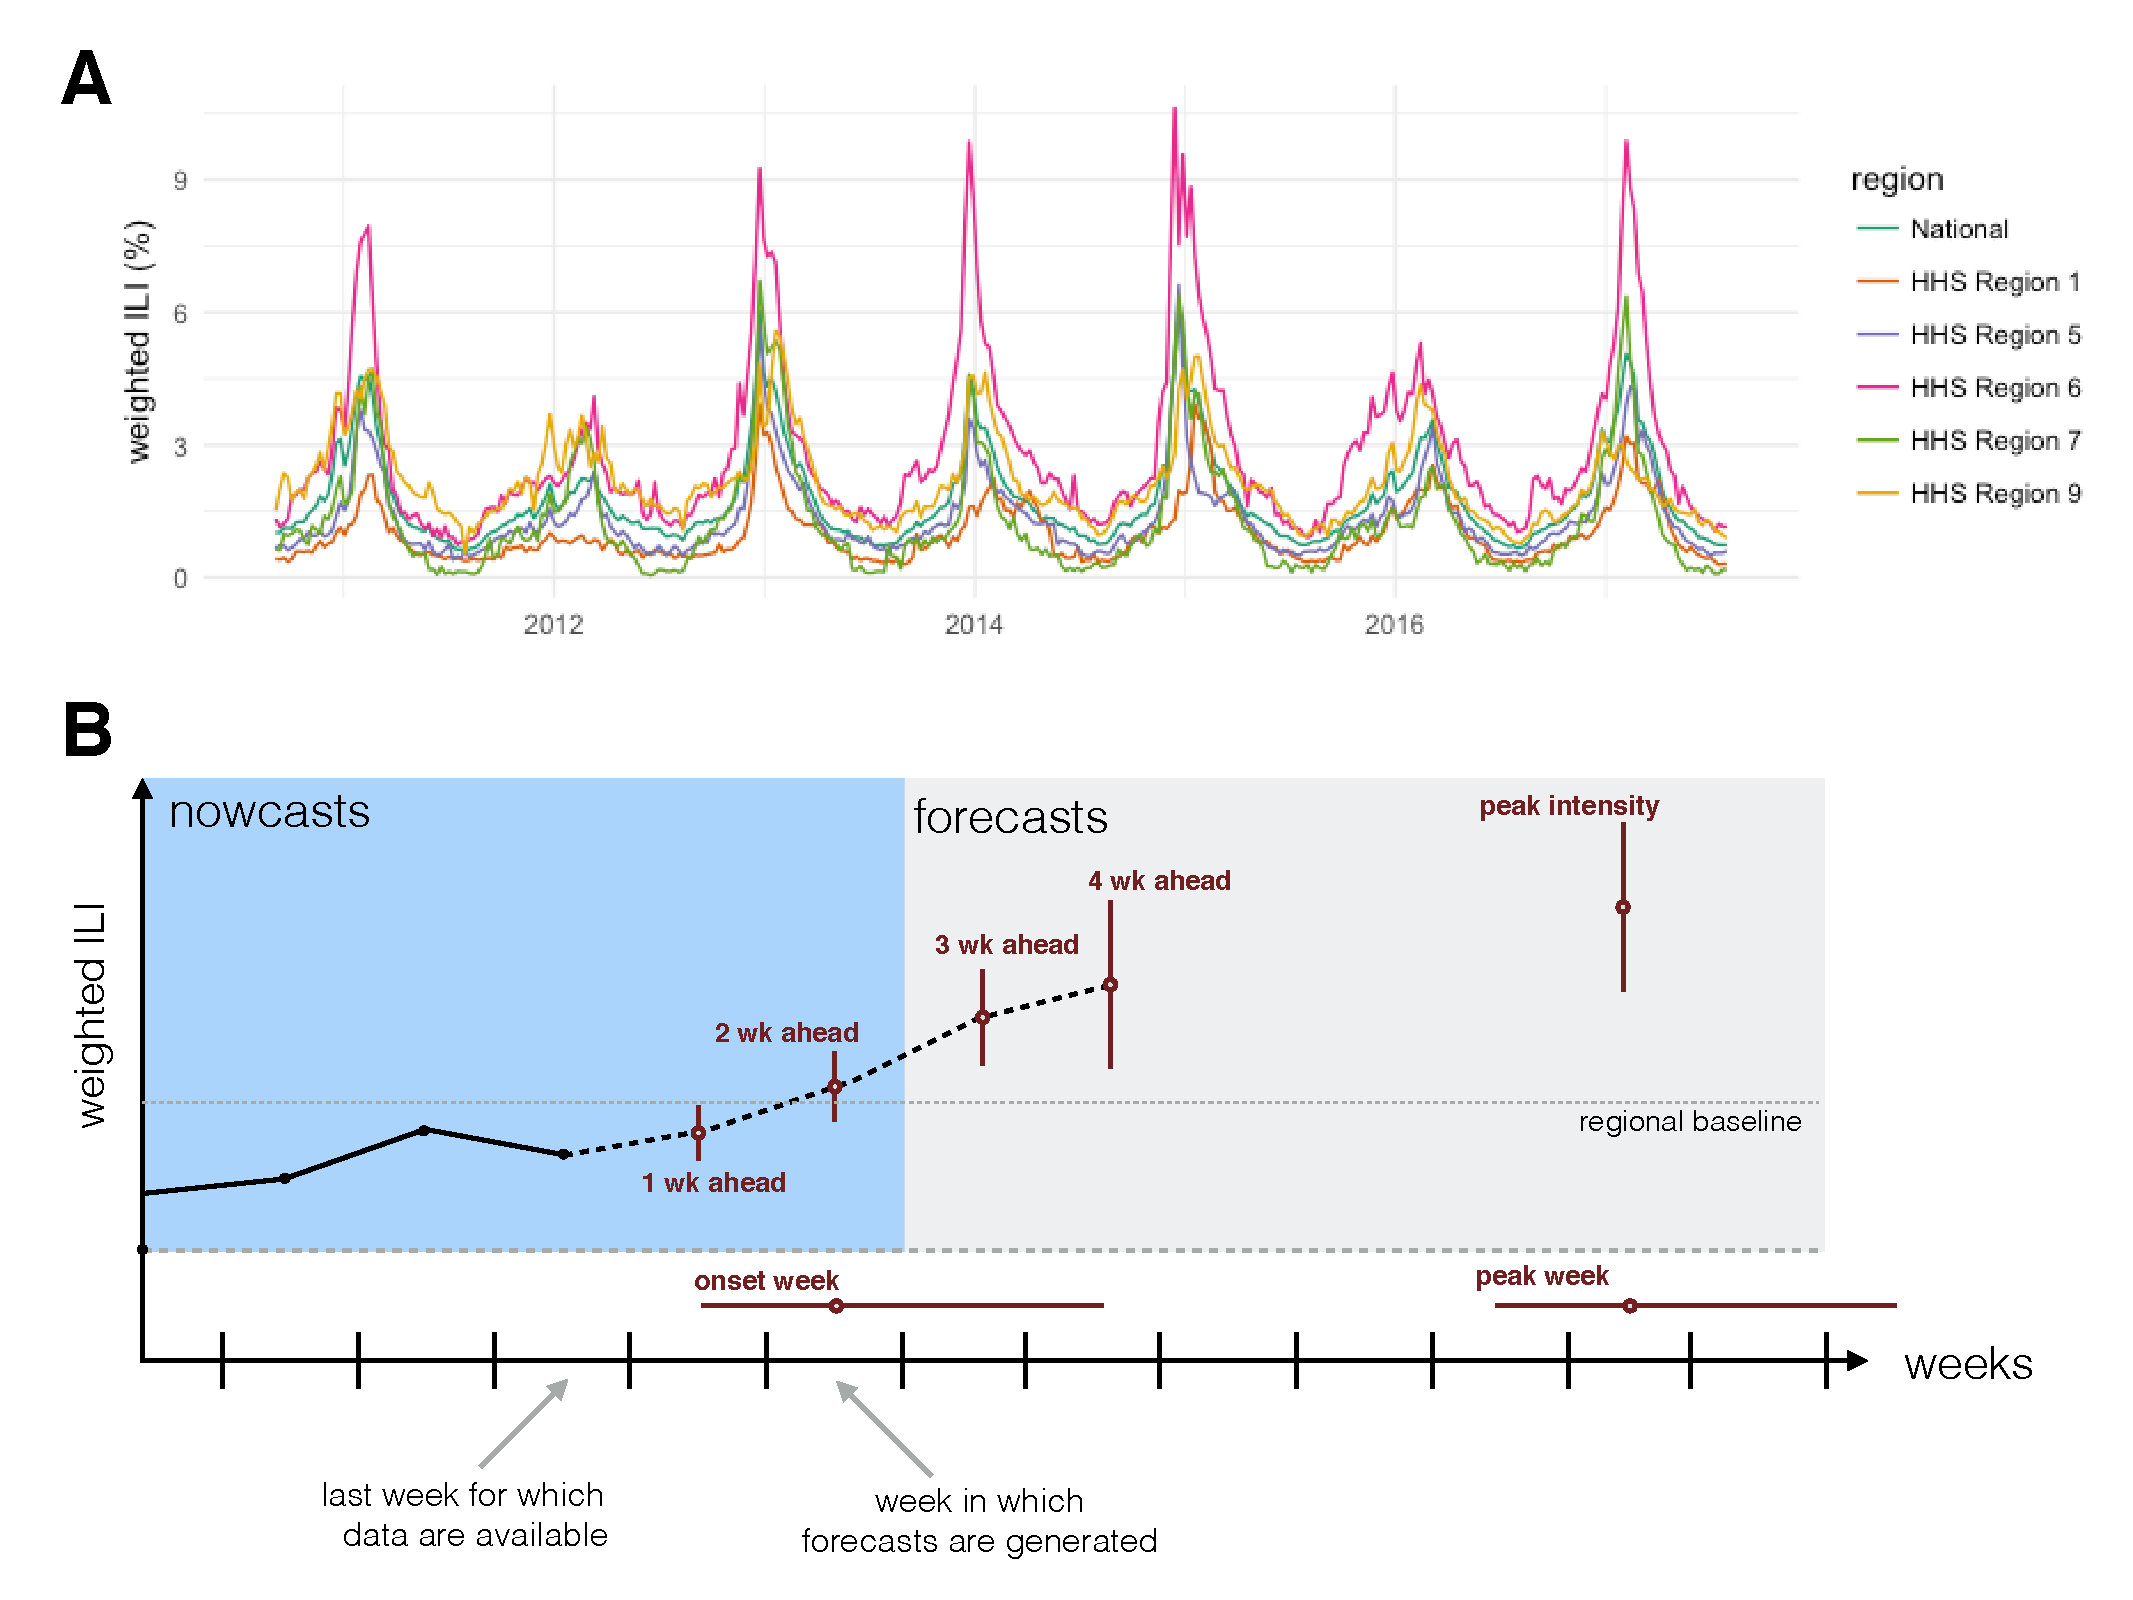
\includegraphics[width=\linewidth]{static-figures/timezero-sketch.pdf}
\caption{(A) Weighted influenza-like illness data downloaded from the CDC website from selected regions. The y-axis shows the weighted percentage of doctor's office visits in which a patient presents with influenza-like illness for each week from September 2010 through July 2017, which is the time period for which the models presented in this paper made seasonal forecasts. (B) A diagram showing the anatomy of a single forecast. The seven forecasting targets are illustrated with a point estimate (dot) and interval (uncertainty bars). The five targets on the wILI scale are shown with uncertainty bars spanning the vertical wILI axis, while the two targets for a time-of-year outcome are illustrated with horizontal uncertainty bars along the temporal axis. The onset is defined relative to a region- and season-specific baseline wILI percentage defined by the CDC.\cite{biggerstaff2018systematic} Arrows illustrate the timeline for a typical forecast for the CDC FluSight challenge, assuming that forecasts are generated or submitted to the CDC using the most recent reported data. These data include the first reported observations of wILI\% from two weeks prior. Therefore, 1 and 2 week-ahead forecasts are referred to as nowcasts, i.e., at or before the current time. Similarly, 3 and 4 week-ahead forecasts are forecasts, or estimates about events in the future.}
\label{fig:intro-schematic}
\end{figure}

\begin{table}
\setlength{\tabcolsep}{4pt} 
\begin{tabular}{p{1.6cm} l p{7.5cm} l  p{1cm}  p{1cm} p{1cm}}
\hline
Team     & Model Abbr& Model Description & & Ext. Data & Mech. Model & Ens. Model \\ 
\hline
CU       & EAKFC\_SEIRS       & Ensemble Adjustment Kalman Filter SEIRS & \cite{Pei2018}  & x & x & \\ 

~        & EAKFC\_SIRS        & Ensemble Adjustment Kalman Filter SIRS & \cite{Pei2018}  & x & x & \\
~        & EKF\_SEIRS         & Ensemble Kalman Filter SEIRS & \cite{Yang2017}    & x             & x &                    \\
~        & EKF\_SIRS          & Ensemble Kalman Filter SIRS & \cite{Yang2017}     & x             & x   &                 \\
~        & RHF\_SEIRS         & Rank Histogram Filter SEIRS & \cite{Yang2017}    & x             & x     &               \\
~        & RHF\_SIRS          & Rank Histogram Filter SIRS & \cite{Yang2017}     & x             & x       &             \\
~        & BMA                & Bayesian Model Averaging & \cite{Yamana2017}      & ~             & ~          &          \\
\hline
Delphi   & BasisRegression    & Basis Regression ({\tt epiforecast} defaults) & \cite{Brooks2015a} & ~             & ~     &               \\ 
~        & DeltaDensity1      & Delta Density ({\tt epiforecast} defaults)   & \cite{Brooks2015a} & ~             & ~       &             \\ 
~        & EmpiricalBayes1    & Empirical Bayes (conditioning on past four weeks) & \cite{Brooks2015,Brooks2015a} & ~             & ~  &                  \\ 
~        & EmpiricalBayes2    & Empirical Bayes ({\tt epiforecast} defaults) & \cite{Brooks2015,Brooks2015a} & ~             & ~            &        \\ 
~        & EmpiricalFuture    & Empirical Futures ({\tt epiforecast} defaults) &  \cite{Brooks2015a} & ~             & ~         &           \\ 
~        & EmpiricalTraj      & Empirical Trajectories ({\tt epiforecast} defaults)& \cite{Brooks2015a} & ~             & ~         &           \\ 
~        & DeltaDensity2      & Markovian Delta Density ({\tt epiforecast} defaults)& \cite{Brooks2015a} & ~             & ~          &          \\ 
~        & Uniform            & Uniform Distribution&  & ~             & ~   &                 \\ 
~        & Stat               & Ensemble (combination of 8 Delphi models)& & ~             & ~  & x                 \\
\hline
LANL     & DBM                & Dynamic Bayesian SIR Model with discrepancy & \cite{Osthus2017} & ~             & x      &              \\ 
\hline
ReichLab & KCDE               & Kernel Conditional Density Estimation & \cite{Ray2017}  & ~             & ~            &        \\ 
~        & KDE                & Kernel Density Estimation and penalized splines & \cite{Ray2018}  & ~             & ~     &               \\ 
~        & SARIMA1            & SARIMA model without seasonal differencing & \cite{Ray2018} & ~             & ~      &              \\ 
~        & SARIMA2            & SARIMA model with seasonal differencing & \cite{Ray2018} & ~             & ~           &         \\ 
\hline
UTAustin & EDM                & Empirical Dynamic Model, or method of analogues & \cite{Sugihara1990} & ~             & ~         &           \\ 
\end{tabular}
\caption{List of models, with key characteristics. Team abbreviations are translated as: CU = Columbia University, Delphi = Carnegie Mellon, LANL = Los Alamos National Laboratories, ReichLab = University of Massachusetts Amherst, UTAustin = University of Texas Austin.  The `Ext data' column notes models that use data external to the ILINet data from CDC. The `Mech. model' column notes models that rely to some extent on an mechanistic or compartmental model formulation. The `Ens. model' column notes models that are ensemble models.}
\label{tab:model-list}
\end{table}





\section*{Results}


\subsection*{Performance in forecasting week-ahead incidence}

Influenza forecasts have been evaluated by the CDC primarily using a variation of the log-score, a measure that evaluates both the precision and accuracy of a forecast.\cite{Gneiting2007} 
Consistent with the primary evaluation performed by the CDC, we used a modified form of the log-score to evaluate forecasts (see Methods). 
The reported scores are aggregated into an average on the log scale and then exponentiated so the reported scores can be interpreted as the (geometric) average probability assigned to the eventually observed value of each target by a particular model. 
Therefore, higher scores reflect more accurate forecasts. 
As a common reference point, we compare all models to a historical baseline model, {\tt ReichLab-KDE}, which forecasts the same historical average every week within a season and does not update based on recently observed data.



Average score for all of the short term forecasts (1 through 4 week-ahead targets) varied substantially across models and regions (Figure \ref{fig:results-model-region-tt}).
The model with the highest average score for the week-ahead targets across all regions and seasons was {\tt CU-EKF\_SIRS}.
This model achieved a region-specific average forecast score for week-ahead targets between
0.32 
and 
0.55.
As a comparison, the historical baseline model {\tt ReichLab-KDE} achieved between
0.12 and
0.37
average score for all week-ahead targets.
% Of the n_models models available for comparison to the historical baseline, n_above_kde_wkahead
% (specify_decimal(n_above_kde_wkahead/n_models*100)\%) showed greater score than the historical baseline across all region-seasons.

\begin{knitrout}
\definecolor{shadecolor}{rgb}{0.969, 0.969, 0.969}\color{fgcolor}\begin{figure}
\includegraphics[width=\linewidth]{figure/results-model-region-tt-1} \caption[Average forecast score by model region and target-type, averaged over weeks and seasons]{Average forecast score by model region and target-type, averaged over weeks and seasons. The text within the grid shows the score itself. The white midpoint of the color scale is set to be the target- and region-specific average of the historical baseline model, {\tt ReichLab-KDE}, with darker blue colors representing models that have better scores than the baseline and darker red scores representing models that have worse scores than the baseline. The models are sorted in descending order from most accurate (top) to least accurate (bottom) and regions are sorted from high scores (right) to low scores (left).}\label{fig:results-model-region-tt}
\end{figure}


\end{knitrout}


% \begin{figure}[htbp]
% \begin{center}
% \includegraphics[width=\textwidth]{figures/fig-results-region.pdf}
% \caption{Average forecast skill by model region and target-type, averaged over weeks and seasons. The white midpoint of the color scale is set to be the overall average of the historical baseline model, {\tt ReichLab-KDE}.}
% \label{fig:results-region}
% \end{center}
% \end{figure}



% Even within models, week-ahead forecast score showed large region-to-region and year-to-year variation. 
% The forecast score for specific region-seasons shown by the high-accuracy {\tt sanitize(max_logscore_model_wkahead)} model varied from 
% specify_decimal(exp(min(top_model_wkahead_scores)), 2) to
% specify_decimal(exp(max(top_model_wkahead_scores)), 2).

% The model with the lowest variation in combined week-ahead forecast skill across region-seasons (excluding the uniform model) was 
% sanitize(min_logscorevar_model_wkahead), 
% with skills ranging between 
% specify_decimal(exp(min(min_logscorevar_model_wkahead_scores)), 2) and 
% specify_decimal(exp(max(min_logscorevar_model_wkahead_scores)), 2).
% The model with the highest variation in forecast skill across region-seasons was 
% sanitize(max_logscorevar_model_wkahead), 
% with skills ranging between 
% specify_decimal(exp(min(max_logscorevar_model_wkahead_scores)), 2) and 
% specify_decimal(exp(max(max_logscorevar_model_wkahead_scores)), 2).



Models were more consistently able to forecast week-ahead wILI in some regions than in others.
Predictability for a target can be broken down into two components. 
First, what is the baseline score that a model derived solely from historical averages can achieve? 
Second, by using alternate modeling approaches, how much more accuracy can be achieved beyond this historical baseline? 
Looking at results across all models,
%from the length(models_wkahead_better_than_kde) models that on average had more skill than the historical baseline in forecasting week-ahead targets, 
HHS Region 1 was the most predictable and HHS Region 6 was the least predictable (Figure \ref{fig:results-model-region-tt}).








\begin{knitrout}
\definecolor{shadecolor}{rgb}{0.969, 0.969, 0.969}\color{fgcolor}\begin{figure}
\includegraphics[width=\maxwidth]{figure/plot-historical-baseline-comparison-1} \caption[Absolute and relative forecast performance for week-ahead (top row) and seasonal (middle row) targets, summarized across all models that on average performed better than the historical baseline]{Absolute and relative forecast performance for week-ahead (top row) and seasonal (middle row) targets, summarized across all models that on average performed better than the historical baseline. Panels A \& C show maps of the U.S. that illustrate spatial patterns of average forecast accuracy for week-ahead (A) and seasonal (C) targets. Color shading indicates average forecast score for this model subset. Panels B \& D compare historical baseline model score (x-axis) with the average score (y-axis, horizontal dashed line at average across regions) with one point for each region. For example, a y-value of 0.1 indicates that the models on average assigned 10\% more probability to the eventually observed value than the historical baseline model. The digits in the plot refer to the corresponding HHS Region number, with N indicating the US National region. Panel E shows the number of seasons each model had average performance above the historical baseline.}\label{fig:plot-historical-baseline-comparison}
\end{figure}


\end{knitrout}


The models presented show substantial improvements in accuracy compared to forecasts from the historical baseline model in all regions of the US.
Results that follow are based on summaries from those models that on average showed higher forecast score than the historical baseline model.
HHS Region 1 showed the best overall week-ahead predictability of any region. Here, the models showed an average forecast score of 
0.54 
for week-ahead targets (Figure \ref{fig:plot-historical-baseline-comparison}A). 
This means that in a typical season these models assigned an average of 
0.54 
probability to the accurate wILI percentages.
%best_region_wkahead showed the best overall week-ahead predictability of any region (overall average score = 
%specify_decimal(exp(kde_scores_wkahead$avg_logscore[which(scores_by_region_wkahead$Location==best_region_wkahead)]),2)). 
This resulted from having the highest score from the baseline model 
(0.37) 
and having the largest improvement upon baseline predictions 
(0.17)
from the other models (Figure \ref{fig:plot-historical-baseline-comparison}B).  
In HHS Region 6 the average week-ahead score was 
0.24. 
While HHS Region 6 showed the lowest baseline model score of any region
(0.12), 
it also showed the second highest improvement
(0.12)
upon baseline predictions (Figure \ref{fig:plot-historical-baseline-comparison}B).
%This was just marginally better than the week-ahead forecast skill for the historical average model in worst_region_wkahead, which was specify_decimal(kde_kwkahead_worst_score,2).





Forecast score declined as the target moved further into the future relative to the most recent observation.
Over half of the models outperformed the historical baseline model in making 1-week ahead forecasts, as 15 of 22 models outperformed the historical baseline in at least 6 of the 7 seasons.
However, only 7 out of 22 models outperformed the historical baseline in at least 6 seasons when making 4-week ahead forecasts.
For the model with highest forecast score across all four week-ahead targets ({\tt CU-EKF\_SIRS}), the average scores across regions and seasons for 1 through 4 week-ahead forecasts were 
0.55, 
0.44, 
0.36, and 
0.31.
This mirrored an overall decline in score observed across most models.
Only in HHS Region 1 were the forecast scores from the {\tt CU-EKF\_SIRS} model for both the ``nowcast'' targets (1 and 2 weeks ahead) above 0.5.

% The historical baseline model showed an average forecast score of 
% specify_decimal(exp(scores_by_model_target$avg_logscore[which(scores_by_model_target$Model=="ReichLab-KDE" & scores_by_model_target$Target == "1 wk ahead" )]), 2), 
% for all week-ahead targets. 
% (Performance does not decline at longer horizons for the historical baseline model, since its forecasts are always the same for a given week.)
% For 1 week-ahead forecasts, n_models_better_than_kde_1wk of n_models models (specify_decimal(n_models_better_than_kde_1wk/n_models*100)\%) showed higher scores than a historical baseline.
% For the 4 week-ahead forecasts, only n_models_better_than_kde_4wk of n_models models (specify_decimal(n_models_better_than_kde_4wk/n_models*100)\%) showed higher scores than the historical baseline.

\subsection*{Performance in forecasting seasonal targets}




Overall, forecast score was lower for seasonal targets than for week-ahead targets, although the models showed greater relative improvement compared to the baseline model (Figure \ref{fig:results-model-region-tt}).
%While the scale of the log score can depend on the number of possible bins in the predictive distribution (i.e., more bins means less probability on average assigned to each bin), the model that assigned uniform probabilities to all possible outcomes achieved similar forecast skill for both seasonal and week-ahead targets.
%This shows that as a whole, the models performed worse on predicting seasonal targets relative to this uniform baseline.
The historical baseline model achieved  an overall forecast score of 
0.14.
The best single model across all seasonal targets was {\tt LANL-DBM} with an overall forecast score of 
0.36, more than a two-fold increase in score over the baseline.



Of the three seasonal targets, models showed the lowest average score in forecasting season onset, with an overall average score of 
0.15. 
Due to the variable timing of season onset, different numbers of weeks were included in the final scoring for each region-season (see Methods). 
%, varying from XX to XX weeks per region-season .
Of the 77 region-seasons evaluated, 9 had no onset, i.e., the wILI did not remain above a fixed region-specific threshold of influenza activity for three or more weeks (see Methods for details). 
The best model for onset was 
{\tt LANL-DBM}, 
with an overall average score of 
0.33
and region-season-specific scores for onset that ranged from
0.03 to 
0.81.
The historical baseline model showed an average score of 
0.11 in forecasting onset.
%Overall, n_above_kde_onset of n_models models (round(n_above_kde_onset/n_models*100)\%) had higher average forecast score than the historical baseline model in the scoring period of interest.
Overall, 8 out of 22 models (36\%) had better overall score for onset in at least 6 out of the 7 seasons evaluated (Figure \ref{fig:plot-historical-baseline-comparison}E).

Accuracy in forecasting season onset was also impacted by revisions to wILI data. In some region-seasons current data led models to be highly confident that onset had occurred in one week, only to have revised data later in the season change the week that was considered to be the onset. One good example of this is HHS Region 2 in 2015/2016. Here, data in early 2016 showed season onset to be EW2 of 2016. Revisions to the data around EW12, led the models to identify EW51 as the onset. A further revision, occurring in EW21 of 2016, showed the onset actually occurred on EW4 of 2016.
Networked metapopulation models that take advantage of observed activity in one location to inform forecasts of other locations have shown promise for improving forecasts of season onset.\cite{Pei2018}



Models showed an overall average score of 
0.23
in forecasting peak week. 
The best model for peak week was 
{\tt ReichLab-KCDE}, 
with an overall average score of 
0.35. 
Region- and season-specific forecast score from this model for peak week ranged from
0.01 to 
0.67.
The historical baseline model showed 
0.17 
score in forecasting peak week.
%Overall, n_above_kde_pkwk of n_models models (round(n_above_kde_pkwk/n_models*100)\%) had higher overall forecast score than the historical baseline model in the scoring period of interest.
Overall, 15 out of 22 models (68\%) had better overall score for peak week in at least 6 out of the 7 seasons evaluated (Figure \ref{fig:plot-historical-baseline-comparison}E).

Models showed an overall average score of 
0.20
in forecasting peak intensity. 
The best model for peak intensity was 
{\tt LANL-DBM}, 
with overall average score of 
0.38. 
Region- and season-specific forecast scores from this model for peak intensity ranged from
0.13 to 
0.61.
The historical baseline model showed 
0.13 
score in forecasting peak intensity.
%Overall, n_above_kde_pk of n_models models (round(n_above_kde_pk/n_models*100)\%) had higher overall forecast score than the historical baseline model in the scoring period of interest for peak intensity.
Overall, 12 out of 22 models (55\%) had better overall score in at least 6 out of the 7 seasons evaluated (Figure \ref{fig:plot-historical-baseline-comparison}E).

% For example, the peak intensity and peak week scores for each model could also be reported (a) early in the season; (b) in the 4-6 weeks prior to the peak; (c) in the 4-6 weeks following the peak, and (d) at the end of the season. 

\begin{knitrout}
\definecolor{shadecolor}{rgb}{0.969, 0.969, 0.969}\color{fgcolor}\begin{figure}
\includegraphics[width=\linewidth]{figure/accuracy-around-peak-1} \caption[Average forecast score by model and week relative to peak]{Average forecast score by model and week relative to peak. Scores for each location-season were aligned to summarize average performance relative to the peak week On the x-axis, zero indicates the peak week and positive values represent weeks after the peak week. In general, models that were updating forecasts based on current data showed improved accuracy for peak targets once the peak had passed. Only several of the models consistently assigned probabilities greater than .2 to the eventually observed values prior to the peak week.}\label{fig:accuracy-around-peak}
\end{figure}


\end{knitrout}

While models for peak week and peak percentage converged on the observed values after the peak occurred, prior to the peak occurring all models showed substantial uncertainty (Figure \ref{fig:accuracy-around-peak}). 
For peak percentage, only one model ({\tt LANL-DBM}) assigned on average more than 0.3 probability to within 0.5 wILI units of the eventual value (the criteria used by the CDC for evaluating model accuracy) prior to the peak occurring. At the peak week of the season, four models assigned on average 0.3 or more probability to the eventually observed values. In forecasting peak week, the models were able to forecast the eventual observed value with slightly more certainty earlier than for peak percentage. One week prior to the peak, three models assigned 0.3 or more probability to within 1 week of the observed peak week while at the peak week, 14 models assigned on average 0.3 or more probability to the eventually observed peak week.


% \subsection*{Performance of models by location}
% 
% Consider adding map that averages across all models, or shows max skill per region, as it varies quite a bit.
% 
% two columns: by target type
% mapa: average performance across all models(-KDE)/targets by region
% mapb: performance of historical model by region
% figc: scatter plot of AVERAGE region-level historical model skill on x and avg model skill on y (one point for each region, aggregated across seasons?). Point is to show that regions with higher season-to-season variation (i.e., lower historical forecast skill) also have lower skill from other models? Maybe plot one line for top models, one for all models. 
% 
% Hypothesis: year-to-year variation within a region (as measured by skill -> lower skill = larger variation) is associated with skill of (top) models for that region. 
% lower skill = larger variation --> lower component model skill

\subsection*{Comparing models' forecasting performance by season}



Averaging across all targets and locations, forecast scores varied widely by model and season (Figure \ref{fig:results-model-season}). 
The historical baseline model ({\tt ReichLab-KDE}) showed an average seasonal score of 
0.20, 
meaning that in a typical season, across all targets and locations, this model assigned on average 
0.20 
probability to the eventually observed value. 
The model with the highest average seasonal forecast score 
({\tt Delphi-Stat}) 
and lowest 
({\tt Delphi-EmpiricalBayes2}) 
had scores of 0.37 and 0.07, respectively. 
Of the 22 models, 16 models 
(73\%) 
showed higher average seasonal forecast score than the historical average.
Season-to-season variation was substantial, with 
10 
models having at least one season with greater average forecast score than the 
{\tt Delphi-Stat}
model did.

\begin{knitrout}
\definecolor{shadecolor}{rgb}{0.969, 0.969, 0.969}\color{fgcolor}\begin{figure}
\includegraphics[width=\linewidth]{figure/results-model-season-1} \caption[Average forecast score, aggregated across targets, regions, and weeks, plotted separately for each model and season]{Average forecast score, aggregated across targets, regions, and weeks, plotted separately for each model and season. Models are sorted from lowest scores (left) to highest scores (right). Higher scores indicate better performance. Dots show average scores across all targets, regions, and weeks within a given season. The `x' marks the geometric mean of the seven seasons. The names of compartmental models are shown in bold face. The {\tt ReichLab-KDE} model (italicized red font) is considered the historical baseline model.}\label{fig:results-model-season}
\end{figure}


\end{knitrout}


% \begin{figure}[htbp]
% \begin{center}
% \includegraphics[width=\textwidth]{figures/fig-results-model-season.pdf}
% \caption{Average forecast score, aggregated across targets and plotted separately for each model and season. Models are sorted from least score (left) to most score (right). Dots show average score across all targets and regions for a given season. The x marks the geometric mean of the seven seasons. The names of compartmental models are shown in bold face. The {\\tt ReichLab-KDE} model can be thought of as the historical baseline model.}
% \label{fig:results-model-season}
% \end{center}
% \end{figure}

The six top-performing models utilized a range of methodologies, highlighting that very different approaches can result in very similar overall performance. 
The overall best model was an ensemble model ({\tt Delphi-Stat}) that used a weighted combination of other models from the Delphi group.
Both the {\tt ReichLab-KCDE} and the {\tt Delphi-DeltaDensity1} model utilized kernel conditional density estimation, a non-parametric statistical methodology that is a distribution-based variation on nearest-neighbors regression. 
These models used different implementations and different input variables, but showed similarly strong performance across all seasons.
The {\tt UTAustin-edm} and {\tt Delphi-DeltaDensity2} models also used variants of nearest-neighbors regression, although overall scores for these models were not consistent, indicating that implementation details and/or input variables can impact the performance of this approach.
The {\tt LANL-DBM} and {\tt CU-EKF\_SIRS} models both rely on a compartmental model of influenza transmission; however the methodologies used to fit and forecast were different for these approaches.
%The CU model used an ensemble Kalman filter approach to generate forecasts, while the LANL model sampled from the posterior predictive distribution using Markov chain Monte Carlo (MCMC).
The {\tt ReichLab-SARIMA2} model used a classical statistical time-series model, the seasonal auto-regressive integrated moving average model (SARIMA), to fit and generate forecasts. 
Interestingly, several pairs of models, although having strongly contrasting methodological approaches, showed similar overall performance; e.g., {\tt CU-EKF\_SIRS} and {\tt ReichLab-SARIMA2}, {\tt LANL-DBM} and {\tt ReichLab-KCDE}.


\subsection*{Comparison between statistical and compartmental models} \label{sec:stat-mech}




On the whole, statistical models achieved similar or slightly higher scores as compartmental models when forecasting both week-ahead and seasonal targets, although the differences were small and of minimal practical significance. 
Using the best three overall models from each category, we computed the average forecast score for each combination of region, season, and target (Table \ref{tab:score-by-model-type}). 
For all targets, except 1 week-ahead forecasts and peak intensity, the difference in model score was slight, and never greater than 
0.02.
For 1-week-ahead forecasts, the statistical models had slightly higher scores on average than mechanistic models  
(0.06, on the probability scale). 
%For the three seasonal targets, the difference in model skill was larger, ranging from 
%specify_decimal(min(scores_by_modeltype$diff_model_skill[5:7]), 2) 
%for 
%scores_by_modeltype$Target[5:7][which.min(scores_by_modeltype$diff_model_skill[5:7])] 
% peak week
% to 
% specify_decimal(max(scores_by_modeltype$diff_model_skill[5:7]), 2) 
% for 
% %scores_by_modeltype$Target[5:7][which.max(scores_by_modeltype$diff_model_skill[5:7])] .
% peak intensity.
We note that the 1 week-ahead forecasts from the compartmental models from the CU team are driven by a statistical ``nowcast`` model that uses data from the Google Search application programming interface (API).\cite{Kandula2017}
Therefore, the CU models were not counted as mechanistic models for 1 week-ahead forecasts.
For peak percentage forecasts, the statistical models had slightly higher scores on average than mechanistic models  
(0.05). 
%Therefore, the only compartmental model making 1 week-ahead forecasts was the {\tt LANL-DBM} model. 

% latex table generated in R 3.5.1 by xtable 1.8-3 package
% Tue Dec  4 20:17:56 2018
\begin{table}[ht]
\centering
\begin{tabular}{lrrr}
   \hline 
 & \multicolumn{2}{c}{score} &  \\
target & stat. model & comp. model & diff. \\ 
  \hline
1 wk ahead & 0.49 & 0.43 & 0.06 \\ 
  2 wk ahead & 0.40 & 0.41 & -0.01 \\ 
  3 wk ahead & 0.35 & 0.34 & 0.00 \\ 
  4 wk ahead & 0.32 & 0.30 & 0.02 \\ 
  Season onset & 0.23 & 0.22 & 0.01 \\ 
  Season peak percentage & 0.32 & 0.27 & 0.05 \\ 
  Season peak week & 0.34 & 0.32 & 0.02 \\ 
   \hline
\end{tabular}
\caption{Comparison of the top three statistical models ({\tt Delphi-DeltaDensity1}, {\tt ReichLab-KCDE}, {\tt ReichLab-SARIMA2}) and the top three compartmental models, ({\tt LANL-DBM}, {\tt CU-EKF\_SIRS}, {\tt CU-RHF\_SIRS}) based on best average region-season forecast score. The diff. column represents the difference in the average probability assigned to the eventual outcome for the target in each row. Positive values indicate the top statistical models showed higher average score than the top compartmental models.} 
\label{tab:score-by-model-type}
\end{table}



% Gamma mixed effects regression model on negative log-scores. Need to remove correlation between successive observation.
% 
% strategies to remove correlation between successive scores within a year:
% \begin{itemize}
%     \item smooth/aggregate scores into different sections of the year, possibly reducing the number of and/or correlation between sucessive scores
%     \item smooth spline across years with random effect for model, fixed effects for model-type
%     \item permutation test
% \end{itemize}


%\subsection*{Where do these models fail?}

%In addition to examining where our models perform well, we also identified situations in which where current state-of-the-art forecast models still need improvement. 
%We identify and quantify several of these challenges, including revisions to initially reported data, ....

\subsection*{Delayed case reporting impacts forecast score}\label{sec:delays}
\begin{knitrout}
\definecolor{shadecolor}{rgb}{0.969, 0.969, 0.969}\color{fgcolor}\begin{figure}
\includegraphics[width=\linewidth]{figure/delay-analysis-1} \caption[Model-estimated changes in forecast skill due to bias in initial reports of wILI \%]{Model-estimated changes in forecast skill due to bias in initial reports of wILI \%. The figure shows estimated coefficient values (and 95\% confidence intervals) from a multivariable linear regression using model, week-of-year, target, and a categorized version of the bias in the first reported wILI \% to predict forecast score.  The x-axis labels show the range of bias (e.g. ``(-0.5,0.5]'' represents all observations whose first observations were within $\pm$ 0.5 percentage points of the final reported value). Values to the left of the dashed grey line are observations whose first reported value were lower than the final. Y-axis values of less than zero (the reference category) represent decreases in expected forecast skill. The total number of observations in each category are shown above the x-axis labels.}\label{fig:delay-analysis}
\end{figure}


\end{knitrout}

In the seven seasons examined in this study, wILI percentages were often revised after first being reported. 
The frequency and magnitude of revisions varied by region, and the majority of initial values (nearly 90\%) are within +/- 0.5\% of the final observed value.
For example, in HHS Region 9, over 51\% of initially reported wILI values ended up being revised by over 0.5 percentage points while in HHS Region 5 less than 1\% of values were revised that much. % see abs_bias_gt_.5 
Across all regions, 10\% of observations were ultimately revised by more than 0.5 percentage points.

When the first report of the wILI measurement for a given region-week was revised in subsequent weeks, we observed a corresponding strong negative impact on forecast accuracy.
Larger revisions to the initially reported data were strongly associated with a decrease in the forecast score for the forecasts made using the initial, unrevised data.
Specifically, among the four top-performing non-ensemble models ({\tt ReichLab-KCDE}, {\tt LANL-DBM}, {\tt Delphi-DeltaDensity1}, and {\tt CU-EKF\_SIRS}), there was an average change in forecast score of -0.29 
(95\% CI: 
-0.39,
-0.19
)
when the first observed wILI measurement was between 2.5 and 3.5 percentage points lower than the final observed value, adjusting for model, week-of-year, and target (Figure \ref{fig:delay-analysis}, see Methods for details on regression model).
Additionally, we observed an expected change in forecast score of 
-0.24 
(95\% CI: 
-0.29,
-0.19
)
when the first observed wILI measurement was between 1.5 and 2.5 percentage points higher than the final observed value.
This pattern is similar for under- and over-reported values, although there were more extreme under-reported values than there were over-reported values. 
Finally, some of the variation in region-specific performance could be attributed to the frequency and magnitude of data revisions.


% \begin{figure}[htbp]
% \begin{center}
% \includegraphics[width=\textwidth]{figures/fig-delay-analysis.pdf}
% \caption{Model-estimated changes in forecast score due to bias in initial reports of wILI \%. The figure shows estimated coefficient values (and 95\% confidence intervals) from a multivariable linear regression using model, week-of-year, target, and a categorized version of the bias in the first reported wILI \% to predict forecast score. The model was fit to  The x-axis labels show the range of bias (e.g. ``(-0.5,0.5]'' represents all observations whose first observations were within $\pm$ 0.5 percentage points of the final reported value). Values to the left of the dashed grey line are observations whose first reported value were lower than the final. Y-axis values of less than zero (the reference category) represent decreases in expected forecast score. The total number of observations in each category are shown above the x-axis labels.}
% \label{fig:delay-model-coefs}
% \end{center}
% \end{figure}


% \subsubsection*{Intensity of season not reliably correlated with forecast score}
% 
% We anticipated seeing a relationship between the peak intensity of the season and the observed forecast score for the peak. 
% However, no clear relationship between the peak intensity of the season and the score at forecasting the peak intensity was observed (data not shown).
% [[Need more detail here.]]

% See analysis in code/peak-analysis.R.

% [[Add a paragraph about capturing a holiday spike?]]

% \begin{itemize}
%     \item holiday peak?
%     \item missing a slow descent because of a second outbreak that is lifting the tail up?
% \end{itemize}



\section*{Discussion}

This work presents the first large-scale comparison of real-time forecasting models from different modeling teams across multiple years.
With the rapid increase in infectious disease forecasting efforts, it can be difficult to understand the relative importance of different methodological advances in the absence of an agreed-upon set of standard evaluations.
We have built on the foundational work of CDC efforts to establish and evaluate models against a set of shared benchmarks which other models can use for comparison.
Our collaborative, team science approach highlights the ability of multiple research groups working together to uncover patterns and trends of model performance that are harder to observe in single-team studies.

Seasonal influenza in the US, given the relative accessibility of historical surveillance data and recent history of coordinated forecasting `challenges', is an important testbed system for understanding the current state of the art of infectious disease forecasting models.
Using models from some of the most experienced forecasting teams in the country, this work reveals several key results about forecasting seasonal influenza in the US. 
\begin{itemize}
    \item A majority of models consistently showed higher accuracy than historical baseline forecasts, both in regions with more predictable seasonal trends and those with less consistent seasonal patterns (Figure \ref{fig:plot-historical-baseline-comparison}B, D, E);
    \item A majority of the presented models showed consistent improvement over the historical baseline for 1 and 2 week-ahead forecasts, although fewer models consistently outperformed the baseline model for 3 and 4 week-ahead forecasts (Figure \ref{fig:plot-historical-baseline-comparison}E);
    \item At the presented spatial and temporal resolutions for influenza forecasts, we did not identify substantial or consistent differences between high-performing models that rely on an underlying mechanistic (i.e., compartmental) model of disease transmission and those that are more statistical in nature (Table \ref{tab:score-by-model-type});
    \item Forecast accuracy is significantly degraded in some regions due to initial partially reported real-time data (Figure \ref{fig:delay-analysis}).
\end{itemize}

As knowledge and data about a given infectious disease system improve and become more granular, a common question among domain-area experts is whether mechanistic models will outperform more statistical approaches.
However, the statistical vs. mechanistic model dichotomy is not always a clean distinction in practice.
In the case of influenza, mechanistic models simulate a specific disease transmission process governed by the assumed parameters and structure of the model. 
But observed ``influenza-like illness'' data is driven by many factors that have little to do with pure influenza transmission (e.g., clinical visitation behaviors, the symptomatic diagnosis process, the case reporting process, a data-revision process, etc.). 
Since influenza-like illness data represent an impure measure of actual influenza transmission, purely mechanistic models may be at a disadvantage in comparison to more structurally flexible statistical approaches when attempting to model and forecast influenza-like illness.
To counteract this potential limitation of mechanistic models in modeling noisy surveillance data, many forecasting models that have a mechanistic core also utilize statistical approaches to explicitly or implicitly account for unexplained discrepancies from the underlying model.\cite{Pei2017,osthus2018dynamic}

There are several important limitations to this work as presented.
While we have assembled and analyzed a range of models from experienced influenza forecasting teams, there are large gaps in the types of data and models represented in our library of models.
For example, relatively few additional data sources have been incorporated into these models, no models are included that explicitly incorporate information about circulating strains of influenza, and no model explicitly includes spatial relationships between regions.
Given that several of the models rely on similar modeling frameworks, adding a more diverse set of modeling approaches would be a valuable contribution.
Additionally, while seven seasons of forecasts from 22 models is the largest study we know of that compares models from multiple teams, this remains a less-than-ideal sample size to draw strong conclusions about model performance. 
Since each season represents a set of highly correlated dynamics across regions, few data are available from which to draw strong conclusions about comparative model performance.
Finally, these results should not be used to extrapolate hypothetical accuracy in pandemic settings, as these models were optimized specifically to forecast seasonal influenza.


% From the perspective of model evaluation, there is no external benchmark defined by the CDC (or others) as to what constitutes a `good' or `useful' forecast. 
% While relative comparisons are useful, it could be beneficial to have public health officials declare a given threshold, a forecast score of, for example, 0.7 or better as `useful'.
%    \item no standard methods for evaluating repeated forecasts of the same targets with the same models...

What is the future of influenza forecasting in the US and globally? %Given available data, what levels of model accuracy are theoretically achievable? 
%This work provides concrete evidence of model performance from experienced forecasting. 
%Challenges like CDC's FluSight are immensely important to the advancement of this field and will continue to advance influenza forecasting capabilities for the US and beyond. 
%Infectious disease forecasting is in its infancy and we expect to see continued model improvement through competition, collaboration, and methodological and technological innovation.
While long-run forecast accuracy for influenza will vary based on a variety of factors (including, e.g. data quality, the geographical scale of forecasts, population density of forecasted areas, and consistency of weather patterns over time\cite{dalziel2018urbanization}), we expect to see continued forecast improvement through competition, collaboration, and methodological and technological innovation.
Further analyses that help elucidate factors that drive forecast accuracy in specific settings will be particularly instructive. 
We see particular promise in models that leverage different data sources, such as pathogen-specific and highly localized incidence data.
Additionally, building ensemble models that capitalize on the strengths of a diverse set of individual component models will be critical to improving accuracy and consistency of models in all infectious disease forecasting settings. 
Ensemble forecasting was the motivation behind the creation of the FluSight Network and, while out of scope of this manuscript, will be the topic of future collaborative research for the group.


To advance infectious disease forecasting broadly, a complete enumeration and understanding of the challenges facing the field is critical.
In this work, we have identified and quantified some of these challenges, specifically focusing on timely reporting of surveillance data. 
However, other barriers may be of equal or greater importance to continued improvement of forecasts.
Often, researchers either lack access to or do not know how best to make use of novel data streams (e.g., Internet data, electronic medical health record data). 
Increased methodological innovation in models that merge together an understanding of biological drivers of disease transmission (e.g., strain-specific dynamics and vaccination effectiveness) with statistical approaches to combine data hierarchically at different spatial and temporal scales will be critical to moving this field forward.
From a technological perspective, additional efforts to standardize data collection, format, storage, and access will increase interoperability between groups with different modeling expertise, improve accessibility of novel data streams, and continue to provide critical benchmarks and standards for the field.
Continuing to refine forecasting targets to more closely align with public health activities will improve integration of forecasts with decision-making. 
Recent work from the CDC has developed standardized algorithms to classify the severity of influenza seasons\cite{biggerstaff2018systematic}, which could be used to inform the development of new forecasting targets.

Public health officials are still learning how to best integrate forecasts into real-time decision making.
Close collaboration between public health policy-makers and quantitative modelers is necessary to ensure that forecasts have maximum impact and are appropriately communicated to the public and the broader public health community.  
Real-time implementation and testing of forecasting methods plays a central role in planning and assessing what targets should be forecasted for maximum public health impact.

\matmethods{

\subsection*{FluSight Challenge Overview}
 
Detailed methodology and results from previous FluSight challenges have been published\cite{Biggerstaff2016,Biggerstaff2018}, and we summarize the key features of the challenge here.

%The FluSight challenge focuses on forecasts of the weighted percentage of doctor's office visits where the patient showed symptoms of an influenza-like illness in a particular region. Weighting is done by state population as the data are aggregated to the regional level.
%This is a standard measure of seasonal flu activity, for which public data is available for the US back to the 1997/1998 influenza season (Figure \ref{fig:intro-schematic}A). 
During each influenza season, the wILI data are updated each week by the CDC. When the most recent data are released, the prior weeks' reported wILI data may also be revised. 
The unrevised data, available at a particular moment in time, are available via the DELPHI real-time epidemiological data API beginning in the 2014/2015 season.\cite{DELPHI} 
This API enables researchers to ``turn back the clock'' to a particular moment in time and use the data available at that time. This tool facilitates more accurate assessment of how models would have performed in real-time. 


The FluSight challenges have defined seven forecasting targets of particular public health relevance. Three of these targets are fixed scalar values for a particular season: onset week, peak week, and peak intensity (i.e., the maximum observed wILI percentage). The remaining four targets are the observed wILI percentages in each of the subsequent four weeks (Figure \ref{fig:intro-schematic}B). A season has an onset week when at least three consecutive weeks are above a CDC-defined regional baseline for wILI. The first of these weeks is considered to be the onset week 

The FluSight challenges have also required that all forecast submissions follow a particular format. A single submission file (a comma-separated text file) contains the forecast made for a particular epidemic week (EW) of a season. Standard CDC definitions of epidemic week are used.\cite{NewMexicoDepartmentofHealth,Niemi2015,Tushar2018} Each file contains binned predictive distributions for seven specific targets across the 10 HHS regions of the US plus the national level. Each file contains over 8000 rows and typically is about 400KB in size.

To be included in the model comparison presented here, previous participants in the CDC FluSight challenge were invited to provide out-of-sample forecasts for the 2010/2011 through 2016/2017 seasons.
For each season, files were submitted for epidemic week 40 (EW40) of the first calendar year of the season through EW20 of the following calendar year. 
(For seasons that contained an EW53, an additional file labeled EW53 was included.)
For each model, this involved creating 233 separate forecast submission files, one for each of the weeks in the seven training seasons.
In total, the forecasts represent over 40m rows and 2.5GB of data.
Each forecast file represented a single submission file, as would be submitted to the CDC challenge. 
Each team created their submitted forecasts in a prospective, out-of-sample fashion, i.e., fitting or training the model only on data available before the time of the forecast (see Figure \ref{fig:intro-schematic}). 
All teams used the Delphi epidata API to retrieve ILINet data.\cite{DELPHI}
Some data sources (e.g. wILI data prior to the 2014/2015 season) were not archived in a way that made data reliably retrievable in this ``real-time'' manner. 
In these situations, teams were still allowed to use these data sources with best efforts made to ensure forecasts were made using only data available at the time forecasts would have been made.

\subsection*{Summary of Models}

Five teams each submitted between 1 and 9 separate models for evaluation (Table \ref{tab:model-list}). 
A wide range of methodological approaches and modeling paradigms are included in the set of forecast models.
For example, seven of the models utilize a compartmental structure (e.g. Susceptible-Infectious-Recovered), a model framework that explicitly encodes both the transmission and the susceptible-limiting dynamics of infectious disease outbreaks.
Other less directly mechanistic models use statistical approaches to model the outbreak phenomenon by incorporating recent incidence and seasonal trends.
One model, {\tt Delphi-Stat}, is an ensemble model, a combination of other models from the Delphi team.
%Six models directly incorporate external data (i.e., not just the wILI measurements from the CDC ILINet dataset), including historical humidity data and Google search data.
No team had early access to CDC surveillance data. Every team accessed the data using same API and baseline datasets.
The Columbia University team used data from Google Extended Health Trends API to nowcast for the 1-week ahead target in all of its models. In their six mechanistic models, the nowcast was also used as an observation i.e. as if it were CDC surveillance data. An analysis of results from the 2016/2017 season showed that the forecast quality of these models improved by about 7\%.\cite{Kandula2018} 
Additionally, the Columbia team used daily specific humidity averaged over 24 years (1979–2002) in their 6 mechanistic models. These climatological estimates were calculated from the National Land Data Assimilation System (NLDAS) project-2 dataset.

Three models stand out as being reference models. 
One shared feature of these models is that their forecasts do not depend on observed data from the season being forecasted. 
The {\tt Delphi-Uniform} model always provides a forecast that assigns equal probability to all possible outcomes. 
The {\tt ReichLab-KDE} model yields predictive distributions based entirely on data from other seasons using kernel density estimation (KDE) for seasonal targets and a generalized additive model with cyclic penalized splines for weekly incidence.
The {\tt Delphi-EmpiricalTraj} model uses KDE for all targets.
The `historical baseline` model named throughout the manuscript refers to the {\tt ReichLab-KDE} model.
Because this model represents a prediction that essentially summarizes historical data, we consider this model an appropriate baseline model to reflect historical trends.

We note that some of the models presented here were developed as standalone forecasting models whereas others were developed as components of a larger ensemble system. We define a standalone model as one that is rigorously validated to show optimal performance on its own. Component models could also be optimized, although they could also be developed solely to provide a specific or supplemental signal as part of a larger system. All of the Delphi group’s models except for {\tt Delphi-Stat} were developed as components rather than standalone models. Despite this, some of the Delphi models, in particular, {\tt Delphi-DeltaDensity1}, performed quite well relative to other standalone models. Component models can also provide useful baselines for comparison, e.g. the {\tt Delphi-Uniform} model, which assigns uniform probability to all possible outcomes, and the {\tt Delphi-EmpiricalTraj} model, which creates a seasonal average model that is not updated based on current data.

Once submitted to the central repository, the models were not updated or modified except in four cases to fix explicit bugs in the code that yielded numerical problems with the forecasts. 
(In all cases, the updates did not substantially change the performance of the updated models.)
Re-fitting of models or tuning of model parameters was explicitly discouraged to avoid unintentional overfitting of models.

\subsection*{Metric Used for Evaluation and Comparison}

%Influenza forecasts have been evaluated by the CDC primarily using a variation of the log-score, a measure that enables evaluation of both the precision and accuracy of a forecast.\cite{Gneiting2007} 
The log-score for a model $m$ is defined as $\log f_m(z^*|\bf{x})$ where $f_m(z|\bf{x})$ is the predicted density function from model $m$ for target $Z$ conditional on some data $\bf{x}$, $z^*$ is the observed value of the target $Z$, and $\log$ is the natural logarithm. 
The log-score is a ``proper`` scoring rule, which has the practical implication that linear combinations (i.e., arithmetic means) of log scores will also be proper.\cite{Gneiting2007}

Following CDC FluSight evaluation procedures, we computed modified log-scores for the targets on the wILI percentage scale such that predictions within $\pm$ 0.5 percentage points are considered accurate, i.e., modified log score = $\log \int_{z^* -.5}^{z^* + .5} f_m(z|{\bf{x}})dz$. 
For the targets on the scale of epidemic weeks, predictions within $\pm$ 1 week are considered accurate, i.e., modified log score = $\log \int_{z^* -1}^{z^* + 1} f_m(z|{\bf{x}})dz$. 
While this modification means that the resulting score is not formally a proper scoring rule, some have suggested that improper scores derived from proper scoring rules may, with large enough sample size, have negligible differences in practice.\cite{Gneiting2007} % see especially last paragraph of section 2.3 
Additionally, this modified log score has the advantage of having a clear interpretation and was  motivated and designed by public health officials to reflect an accuracy of practical significance.
Hereafter, we will refer to these modified log scores as simply log scores.

Average log scores can be used to compare models' performance in forecasting for different locations, seasons, targets, or times of season.
In practice, each model $m$ has a set of log scores associated with it that are region-, target-, season-, and week-specific.
We represent one specific scalar log score value as $\log f_{m,r,t,s,w}(z^*|\bf{x})$. 
These values can be averaged across any of the indices to create a summary measure of performance.
For example,
\begin{eqnarray}
LS_{m,\cdot,t,\cdot,\cdot} & = & \frac{1}{N} \sum_{r,s,w} \log f_{m,r,t,s,w}(z^*|{\bf x}) \label{eqn:logscore}
\end{eqnarray}
represents a log score for model $m$ and target $t$ averaged across all regions, seasons and weeks.

While log scores are not on a particularly interpretable scale, a simple transformation enhances interpretability substantially.
Exponentiating an average log score yields a forecast score equivalent to the geometric mean of the probabilities assigned to the eventually observed outcome (or, more specifically for the modified log score, to regions of the distribution eventually considered accurate). 
The geometric mean is an alternative measure of central tendency to an arithmetic mean, representing the $N^{th}$ root of a product of $N$ numbers. 
Using the example from equation (\ref{eqn:logscore}) above, we then have that
\begin{eqnarray}
S_{m,\cdot,t,\cdot,\cdot} &=& \exp \left ( LS_{m,\cdot,t,\cdot,\cdot} \right ) \nonumber \\
& = & \exp \left ( \frac{1}{N} \sum_{r,s,w} \log f_{m,r,t,s,w}(z^*|{\bf x}) \right ) \nonumber \\
 & = & \left ( \prod_{r,s,w}  f_{m,r,t,s,w}(z^*|{\bf x}) \right ) ^{1/N} 
\end{eqnarray}
In this setting, this score $S$ has the intuitive interpretation of being the average probability assigned to the true outcome (where average is considered to be a geometric average).
Throughout the manuscript, we refer to an exponentiated average log score as an average score.
In all cases, we compute the averages arithmetically on the log scale and only exponentiate before reporting and interpreting a final number.
Therefore, all reported average scores can be interpreted as the corresponding geometric means, or as the correponding average probabilities assigned to the true outcome.
%For some summary calculations (e.g., Figure \ref{fig:plot-historical-baseline-comparison}), we used a subset of models that had shown improved performance over the baseline model.

Following the convention of the CDC challenges, we only included certain weeks in the calculation of the average log scores for each target.
This focuses model evaluation on periods of time that are more relevant for public health decision making.
Forecasts of season onset are evaluated based on the forecasts that are received up to six weeks after the observed onset week within a given region.
Peak week and peak intensity forecasts were scored for all weeks in a specific region-season up until the wILI measure drops below the regional baseline level for the final time. 
%(All weeks are scored if wILI never goes above the baseline.)
%Forecasts of season peak and intensity are evaluated through the first forecast received after the weighted ILI goes below the regional baseline for the final time during a given region-season. 
Week-ahead forecasts are evaluated using forecasts received four weeks prior to the onset week through forecasts received three weeks after the weighted ILI goes below the regional baseline for the final time.
In a region-season without an onset, all weeks are scored.
To ensure all calculated summary measures would be finite, all log scores with values of less than -10 were assigned the value -10, following CDC scoring conventions.
This rule was invoked for 2648 scores, or 0.8\% of all scores that fell within the scoring period.
All scores were based on ``ground truth'' values of wILI data obtained as of September 27, 2017.

% \subsection*{Formal comparisons of model performance}
% 
% Model-based comparisons of forecast accuracy are hindered by the high correlation of sequential forecasts and by outlying observations. 
% When observations assign no probability to the eventually observed outcome they have a log-score of $-\infty$.

%Things to confirm: removed weeks that CDC does not score, no onset seasons and multi peak years are handled appropriately

\subsection*{Specific model comparisons}\label{sec:delay-model}

\subsubsection*{Analysis of data revisions}
% from fig-delay-model-coefs.R
% fm4 <- glm(exp(multi_bin_score) ~ Model + Target + factor(forecasted_epiweek) + bias_first_report_factor, data=scores_for_analysis)

The CDC publicly releases data on doctor's office visits due to ILI each week. 
These data, especially for the most recent weeks, are occasionally revised, due to new or updated data being reported to the CDC since their last publication.
While often these revisions are fairly minor or non-existent, at other times, these revisions can be substantial, changing the reported wILI value by over 50\% of the originally reported value.
Since the unrevised data are used by forecasters to generate current forecasts, real-time forecasts can be biased by the initially reported, preliminary data.

We used a regression model to analyze the impact of these unrevised reports on forecasting.
Specifically, for each region and epidemic week we calculated the difference between the first and the last reported wILI values for each epidemic week for which forecasts were generated in the seven seasons under consideration.
We then created a categorical variable ($X$) with a binned representation of these differences using the following six categories covering the entire range of observed values: (-3.5,-2.5], (-2.5,-1.5], ..., (1.5,2.5].
Using the forecasting results from the four most accurate individual non-ensemble models, ({\tt ReichLab-KCDE}, {\tt LANL-DBM}, {\tt Delphi-DeltaDensity1}, {\tt CU-EKF\_SIRS}), we then fit the following linear regression model
\begin{equation}
S_i = \beta + \alpha_{m(i)} + \gamma_{t(i)} + \lambda_{w(i)} + {\mathbf \theta}\cdot X_i + \epsilon_i
\end{equation}
where $S_i$ is the score, the index $i$ indexes a specific set of subscripts $\{m,r,t,s,w\}$, and the $\alpha_{m(i)}$, $\gamma_{t(i)}$, and $\lambda_{w(i)}$ are model-, target-, and week-specific fixed effects, respectively. (The notation $m(i)$ refers to the model contained in the $i$th observation of the dataset.) The error term is assumed to follow a Gaussian distribution with mean zero and an estimated variance parameter. 
The parameter of interest in the model is the vector ${\mathbf \theta}$, which represents the average change in score based on the magnitude of the bias in the latest available wILI value, adjusted for differences based on model, target, and week-of-season.  The $[-0.5,+0.5]$ change category was taken as a baseline category and the corresponding $\theta$ entry constrained to be 0, so that other $\theta$ entries represent deviations from this baseline.
%the expected changes in average score from the reference category (defined as the bin representing changes of between $\pm$ 0.5 from the original reported value) adjusting for model, target and week-of-season.

\subsubsection*{Mechanistic vs. statistical models}

% Infectious disease modeling has proven to be fertile ground for statisticians, mathematicians, and quantitative modelers for over a century. 
There is not a consensus on a single best modeling approach or method for forecasting the dynamic patterns of infectious disease outbreaks in both endemic and emergent settings. 
Semantically, modelers and forecasters often use a dichotomy of mechanistic vs. statistical (or `phenomenological') models to represent two different philosophical approaches to modeling.
Mechanistic models for infectious disease consider the biological underpinnings of disease transmission, and in practice are implemented as variations on the Susceptible-Infectious-Recovered (SIR) model. 
Statistical models largely ignore the biological underpinnings and theory of disease transmission and focus instead on using data-driven, empirical and statistical approaches to make the best forecasts possible of a given dataset, or phenomenon. 

However, in practice, this dichotomy is less clear than it is in theory.
For example, statistical models for infectious disease counts may have an autoregressive term for incidence (e.g., as done by the {\tt ReichLab-SARIMA1} model).
This could be interpreted as representing a transmission process from one time period to another.
In another example, the {\tt LANL-DBM} model has an explicit SIR compartmental model component but also utilizes a purely statistical model for the discrepancy of the compartmental model with observed trends.
The models from Columbia University used a statistical `nowcasting' approach for their 1-week ahead forecasts, but after that relied on different variations of an SIR model.
% Both approaches are commonly used and both have advantages and disadvantages in different settings.  

We categorized models according to whether or not they had any explicit compartmental framework (Table \ref{tab:model-list}). 
We then took the top three performing compartmental models (i.e., models with some kind of an underlying compartmental structure) and compared their performance with the top three individual component models without compartmental structure. 
We excluded multi-model ensemble models (i.e., {\tt Delphi-Stat}) from this comparison and also excluded the 1 week-ahead forecasts of the CU models from the compartmental model category, since they were generated by a statistical nowcast.
Separately for each target, we compared the average score of the top three compartmental models to the average score of the top three non-compartmental models.

\subsection*{Reproducibility and data availability}

To maximize the reproducibility and data availability for this project, the data and code for the entire project (excluding specific model code) are publicly available.
The project is available on GitHub\cite{fsngithub2018}, with a permanent repository stored on Zenodo\cite{fsnzenodo2018}.
All of the forecasts may be interactively browsed on the website \url{http://flusightnetwork.io}.
A web applet with interactive visualizations of the model evaluations is available at \url{https://reichlab.shinyapps.io/FSN-Model-Comparison/}. 
Additionally, this manuscript was dynamically generated using R version 3.5.1 (2018-07-02), Sweave, and knitr, which are tools for intermingling manuscript text with R code that run the central analyses and minimize the chance for errors in transcribing or translating results.\cite{Xie2015,RCore2017}.

}

\showmatmethods{}

\acknow{The findings and conclusions in this report are those of the authors and do not necessarily represent the official position of the Centers for Disease Control and Prevention, Defense Advanced Research Projects Agency, Defense Threat Reduction Agency, the National Institutes of Health, National Science Foundation, or Uptake Technologies.}

\showacknow{}


\bibliography{../flusightnetwork}

\end{document}
